\documentclass[entwurf.tex]{subfiles}

\begin{document}

\chapter{Sequenzdiagramme}
	\section{Verbindung zwischen Client und Server herstellen}
	\label{Sequence:TerminalConnect}
		In dem folgenden Diagramm sieht man den Ablauf vom Verbinden eines Endgeräts mit dem Server. Darauf folgt normalerweise ''\nameref{Sequence:LiveDataNewConfig}''
		
		Hierbei handelt es sich beim Terminal um das Endgerät auf dem über einen Browser die Vinjab-Seite aufgerufen wird. Der Befehl openWebpage() soll das Aufrufen der Website darstellen. Es handelt sich sozusagen um eine Anfrage, über HTTP, zuerst nach der HTML-Datei. Dann nach den genutzten JavaScript- und CSS-Dateien.

		Das Hypertext Transfer Protocol ist ein Protokoll zur Übertragung von Daten auf der Anwendungsschicht über ein Rechnernetz und gehört dementsprechend zur Internetprotokollfamilie. Es wird hauptsächlich eingesetzt, um Webseiten aus dem Internet in einen Webbrowser zu laden. Es ist jedoch nicht prinzipiell darauf beschränkt und auch als allgemeines Dateiübertragungsprotokoll sehr verbreitet.
		
		Bei der Referenz für die WebRTC-Connection wird ''\nameref{Sequence:WebRTCConnect}'' ausgeführt.
		
		\begin{figure}[H]
 			\makebox[\textwidth][c]{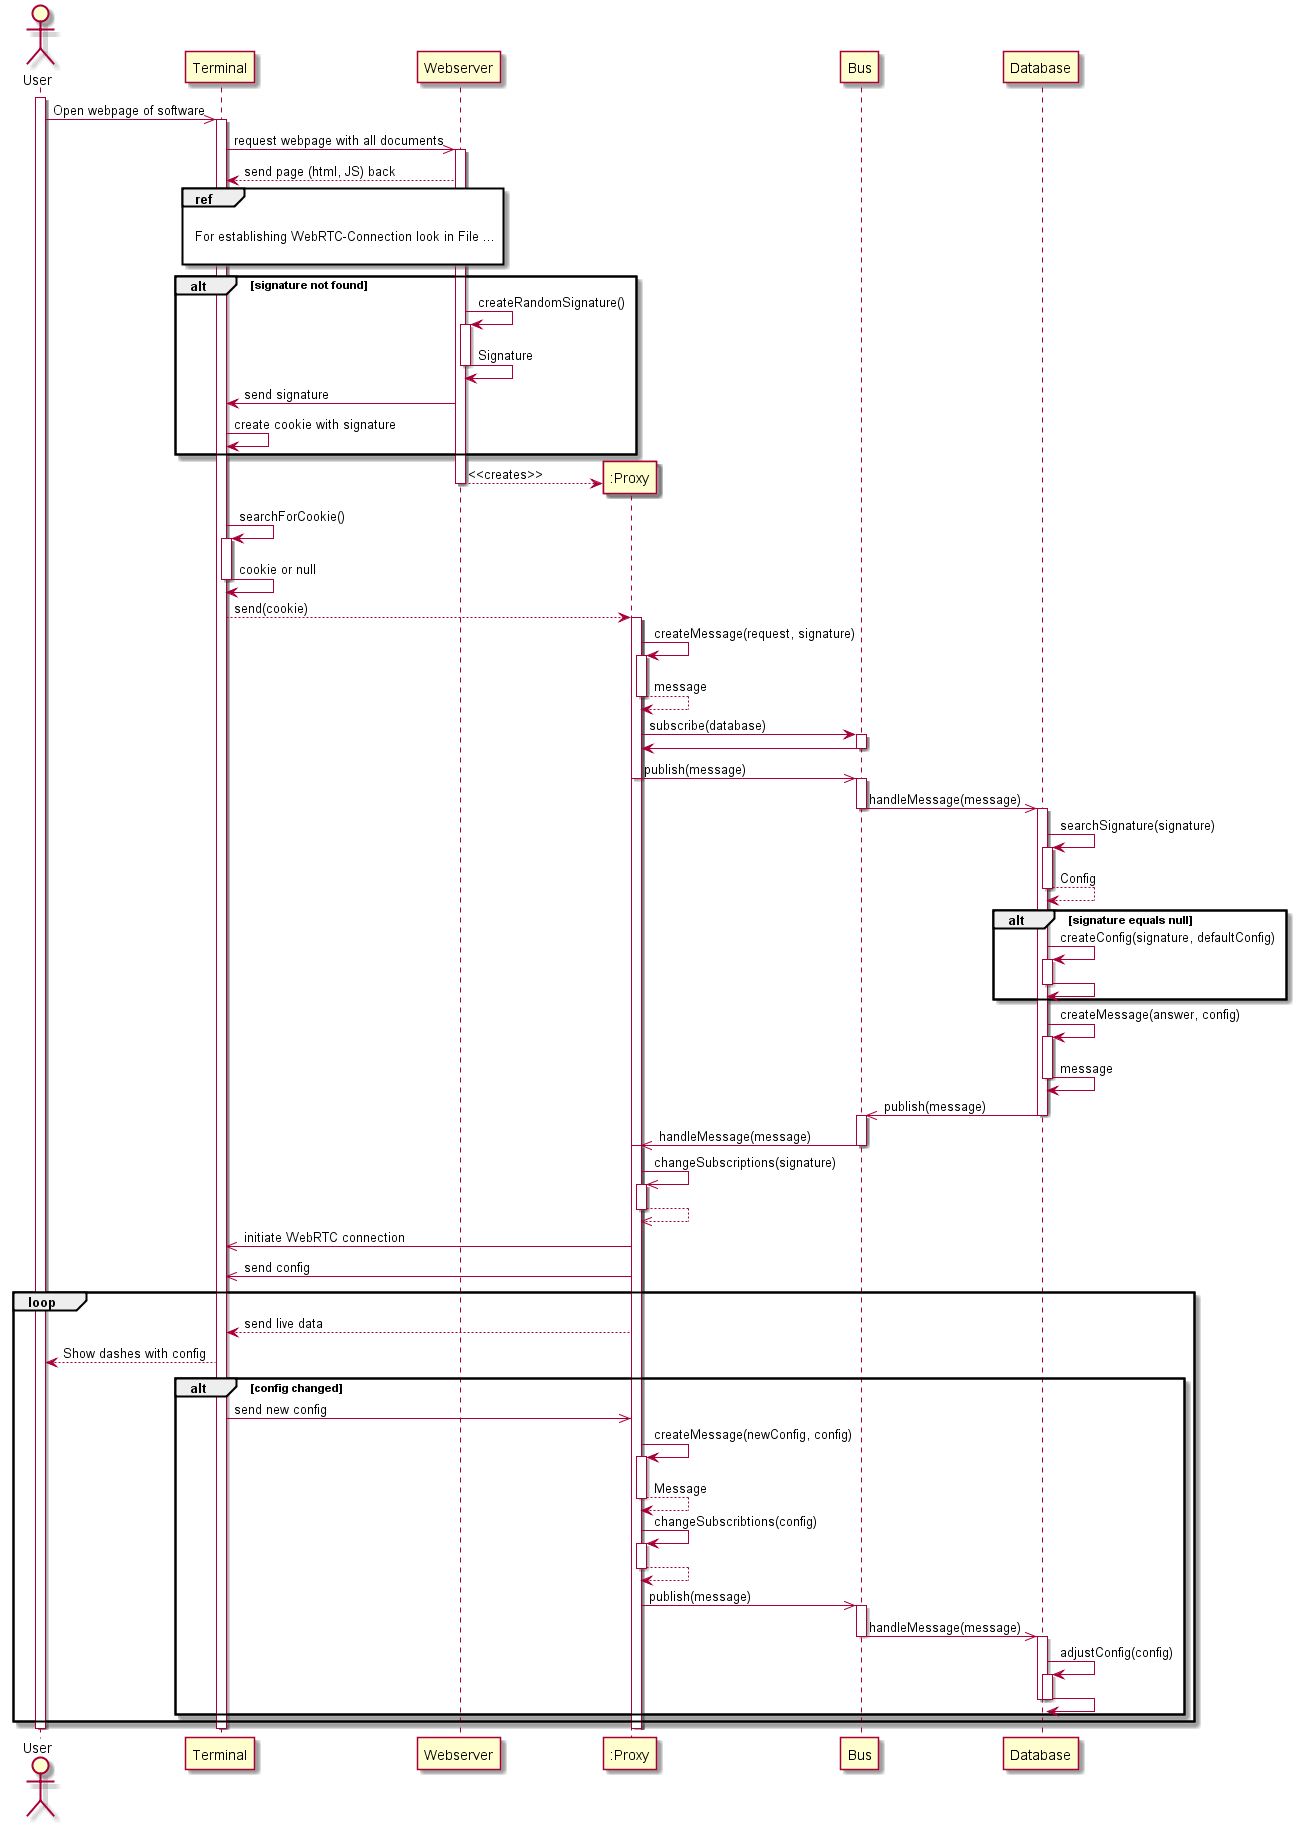
\includegraphics[width=0.9\paperwidth]{diagrams/Connect.png}}
  			\caption{Herstellen einer Verbindung von Client zu Server}
  		\end{figure}
  		
  	\section{WebRTC Verbindung herstellen}
  	\label{Sequence:WebRTCConnect}
		In dem folgenden Diagramm wird dargestellt wie eine WebRTC-Verbindung zwischen dem Endgerät und dem Webserver hergestellt wird. Bei unserem Projekt initiiert der Client die Verbindung. Der Server akzeptiert diese nur.
		
		WebRTC ist eine Sammlung von Kommunikationsprotokollen und Programmierschnittstellen (API) für die Implementierung in Webbrowsern, die diesen Echtzeitkommunikation über Rechner-Rechner-Verbindungen ermöglichen. Damit können Browser nicht mehr nur Datenressourcen von Backend-Servern abrufen, sondern auch (Echtzeitinformationen) von Browsern anderer Benutzer.
		
		\begin{figure}[H]
			\begin{center}
	 			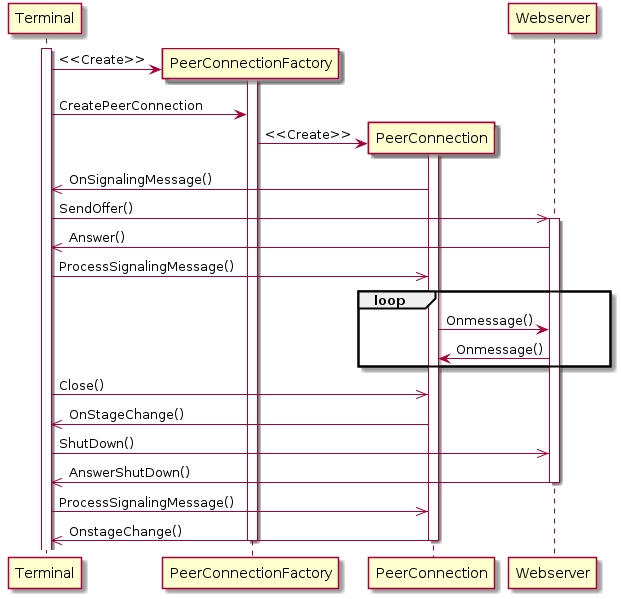
\includegraphics[width=\textwidth]{diagrams/DataTransferSequenz.png}
  				\caption{Herstellen einer WebRTC-Verbindung}
  			\end{center}
  		\end{figure}
  		
  	\newpage
  	\section{Live Daten und neue Konfiguration}
  	\label{Sequence:LiveDataNewConfig}
  		Nach hergestellter Verbindung befindet sich das System in einer Schleife in der eigentlich nur noch Live-Daten vom Server zum Client geschickt werden. Nur wenn der Nutzer die Anzeigeeinstellungen ändert wird diese Schleife für kurze Zeit unterbrochen um die neue Konfiguration an den Server zu übermitteln. Damit von diesem keine nicht benötigten Daten mehr geschickt werden und diese Konfiguration permanent gespeichert, also bei Neustart wieder aufgerufen, werden kann.
  		\begin{figure}[H]
  			\begin{center}
 				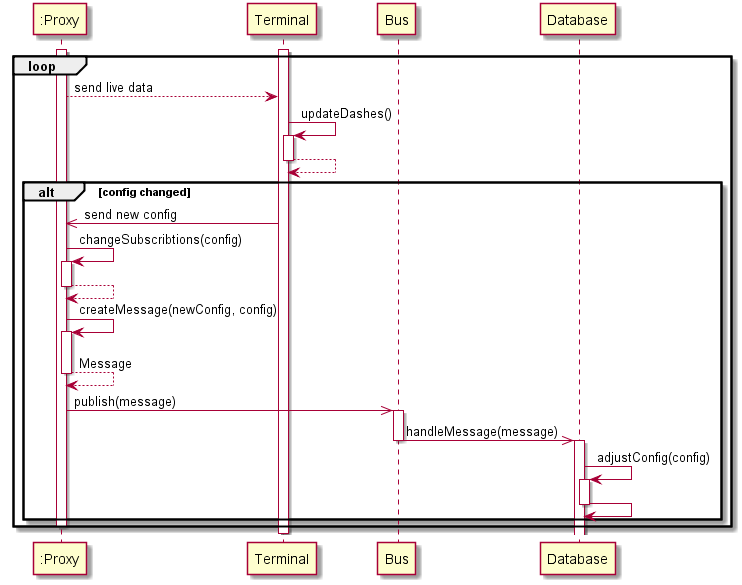
\includegraphics[width=\textwidth]{diagrams/ChangeDashConfig.png}
  				\caption{Live Datenübertragung und Konfigurationsänderung}
  			\end{center}
  		\end{figure}
  		
  	\section{Statistik übertragen}
  		
  		\begin{figure}[H]
 			\makebox[\textwidth][c]{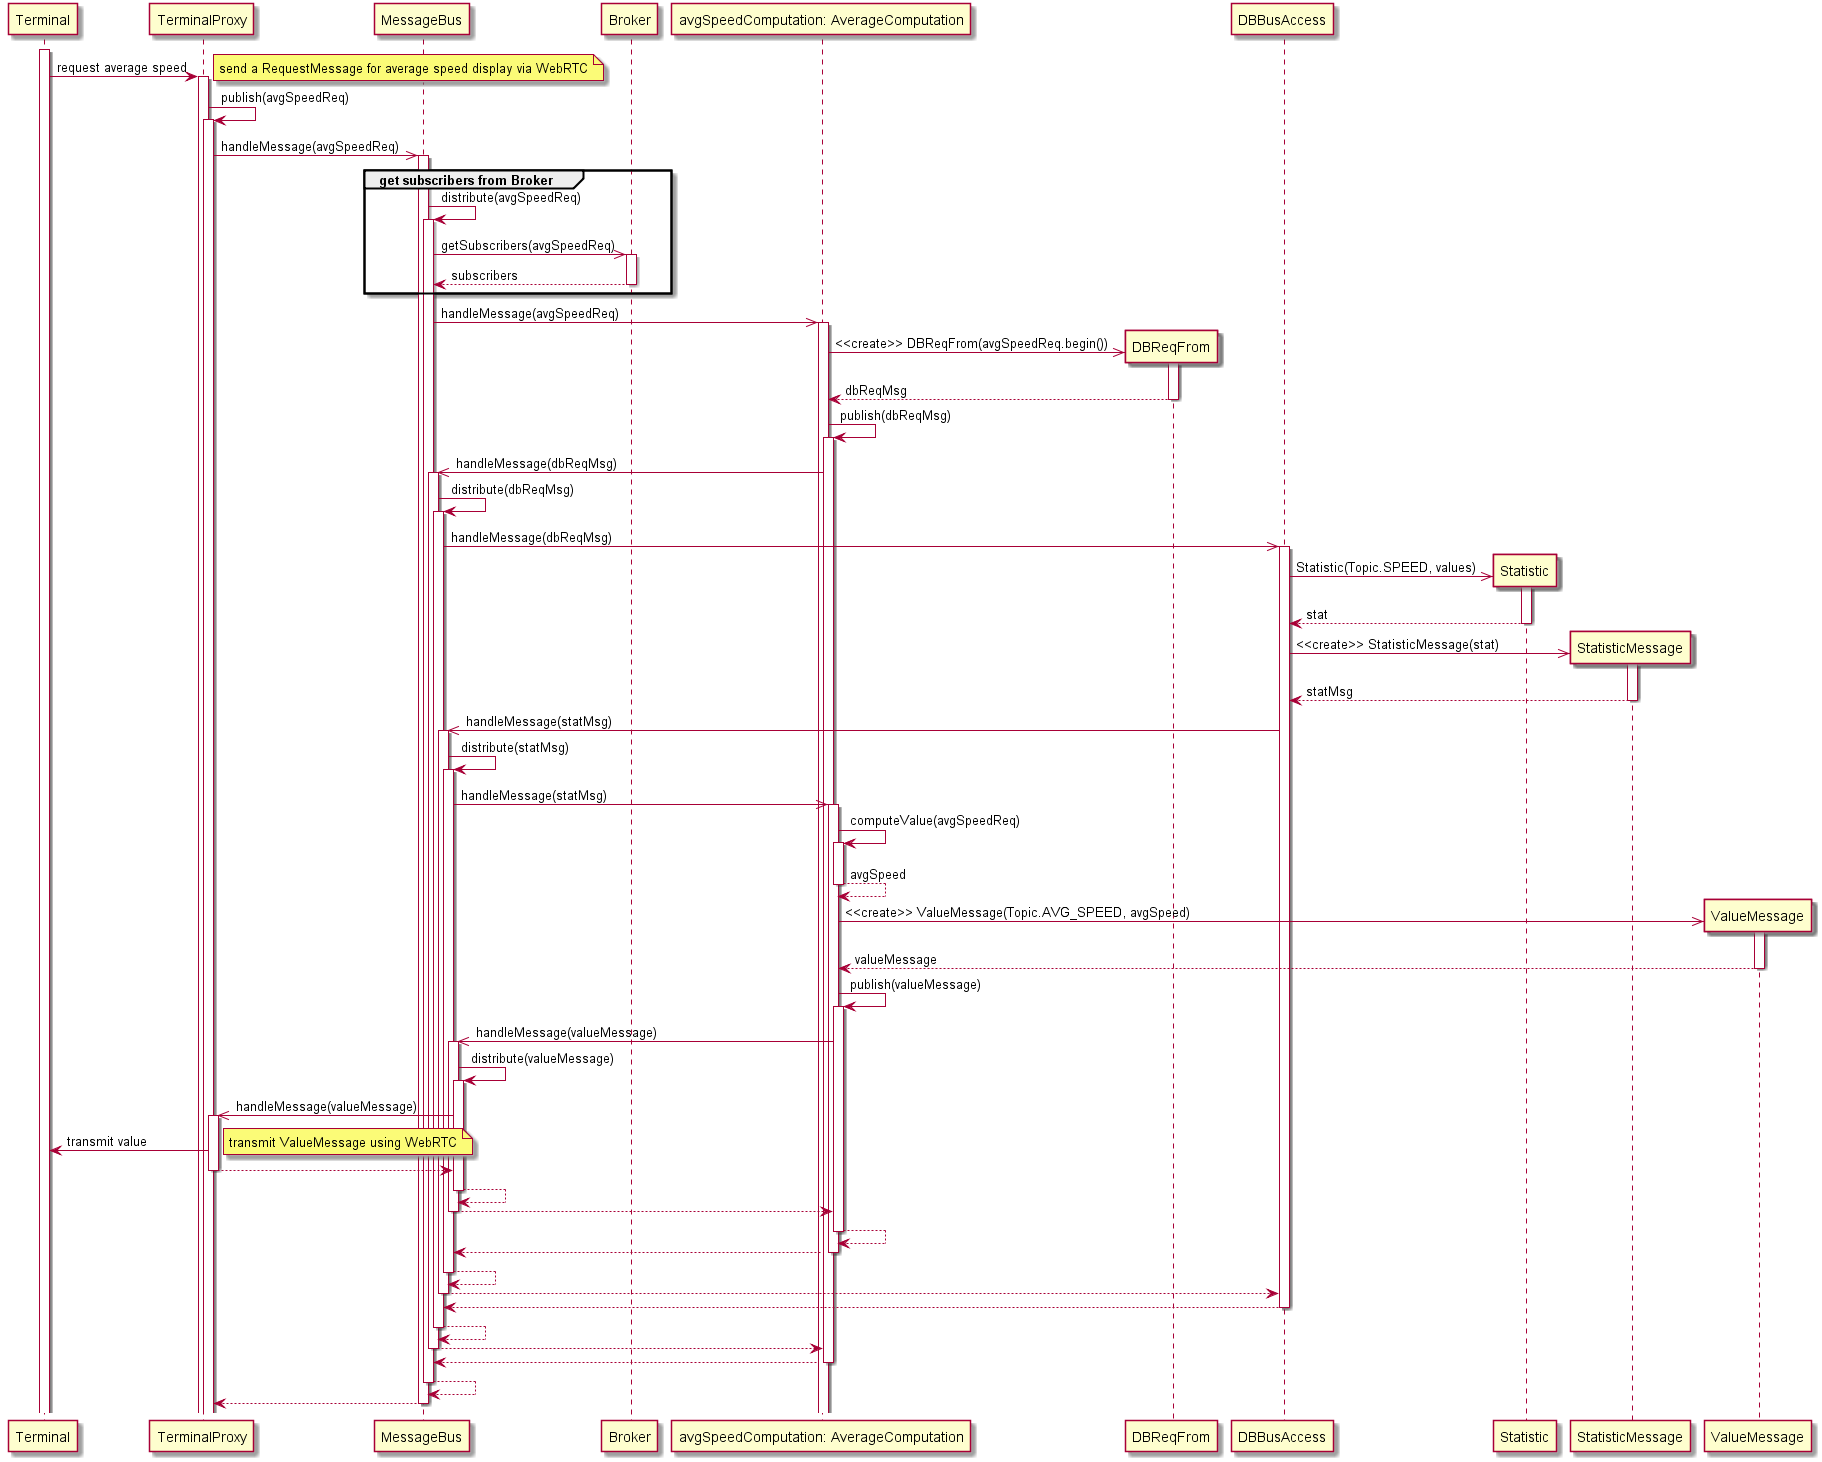
\includegraphics[width=0.9\paperwidth]{diagrams/StatsDBSeq.png}}
  			\caption{Verschiedene Dash-Anzeigeelemente.}
  		\end{figure}
  		
  	
\end{document}